\title{Question 1}
\author{LJ Brown}
%\date{\today}

\documentclass[12pt]{article}
\usepackage{pgf, tikz}
\usetikzlibrary{arrows, automata}
\usepackage{amsmath}
\usepackage{blkarray}

\begin{document}
\maketitle

\section{Question}
1.	(25/25 points) Consider the following web pages and the set of web pages that they link to:
Page A points to pages B and C.
Page B points to page C.
All other pages have no outgoing links.
Apply the PageRank algorithm to this subgraph of pages. Assume $\alpha$ = 0.15. Simulate the algorithm for three iterations. 


% Web Graph
\begin{center}Disconnected Webgraph \end{center}

\begin{center}
	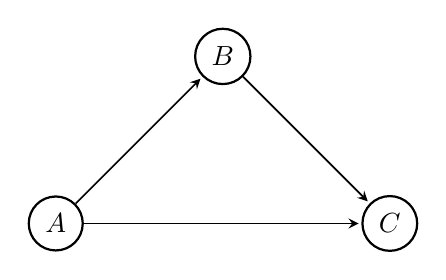
\begin{tikzpicture}[
            > = stealth, % arrow head style
            shorten > = 1pt, % don't touch arrow head to node
            auto,
            node distance = 3cm, % distance between nodes
            semithick % line style
        ]

        \tikzstyle{every state}=[
            draw = black,
            thick,
            fill = white,
            minimum size = 4mm
        ]

        \node[state] (A) {$A$};
        \node[state] (B) [above right of=A] {$B$};
        \node[state] (C) [below right of=B] {$C$};

        \path[->] (A) edge node {} (B);
        \path[->] (A) edge node {} (C);
        \path[->] (B) edge node {} (C);


        %\draw[red, dashed] (1, 2) -- (1, -2);
    \end{tikzpicture}
     \footnote{Webpage C, in the "Disconnected Webgraph" is called a "dangling node".}
\end{center}

\section{PageRank Algorithm}

%
% Idea
%
The "pageRank algorithm" attempts to gauge the importance of each website in a webgraph by ranking each node according to the number and "quality" of its inlinks.

Imagine a web surfer who begins at some webpage or node in the "Disconnected Webgraph" above, and performs a random walk by clicking on different links. At every node the surfer picks a random outlink or edge to follow, each outlink from the same webpage having an equal chance being selected. In the "Disconnected Webgraph" above, the surfer will eventually become trapped at node $C$. 

The "pageRank algorithm" removes the "dangling node" trap by adding connections to nodes with no outlinks to every single other node in the graph. By connecting the "dangling nodes" to every other node, not only would the surfer be able to click forever, but the surfer would continue to revisit every single node in the graph during this infinite walk. 

% Corrected Webgraph
\begin{center}Strongly Connected Webgraph \end{center}

\begin{center}
	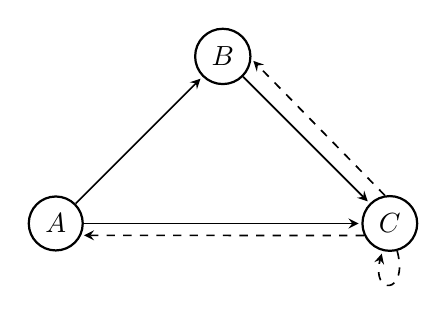
\begin{tikzpicture}[
            > = stealth, % arrow head style
            shorten > = 1pt, % don't touch arrow head to node
            auto,
            node distance = 3cm, % distance between nodes
            semithick % line style
        ]

        \tikzstyle{every state}=[
            draw = black,
            thick,
            fill = white,
            minimum size = 4mm
        ]

        \node[state] (A) {$A$};
        \node[state] (B) [above right of=A] {$B$};
        \node[state] (C) [below right of=B] {$C$};

        \path[->] (A) edge node {} (B);
        \path[->] (A) edge node {} (C);
        \path[->] (B) edge [align=center,below] node {} (C);
        
        % added
        \path[->, dashed] (C) edge [loop below] node {} (C);
        \path[->, dashed] (C.100) edge  node {} (B.-5);
        \path[->, dashed] (C.205) edge node {} (A.-25);

    \end{tikzpicture}
\end{center}

However, although the surfer would eventually revisit every single website, the probability that any particular website is visited next may be different. This probability is the websites "rank". 
%As the surfer approaches an infinite amount of clicks, regardless of the surfers starting point, a websites rank will always be the same. 

A nodes rank, $r_i$, is defined by summing the inlink values of all nodes pointing to it,

\begin{equation}
	\nonumber r_i = \sum_{k \rightarrow i} \frac{r_k}{o_k}
\end{equation}

Where $o_k$ is the number of outlinks for node $k$.

\begin{center}
	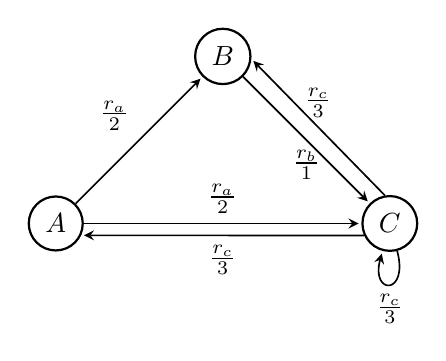
\begin{tikzpicture}[
            > = stealth, % arrow head style
            shorten > = 1pt, % don't touch arrow head to node
            auto,
            node distance = 3cm, % distance between nodes
            semithick % line style
        ]

        \tikzstyle{every state}=[
            draw = black,
            thick,
            fill = white,
            minimum size = 4mm
        ]

        \node[state] (A) {$A$};
        \node[state] (B) [above right of=A] {$B$};
        \node[state] (C) [below right of=B] {$C$};

        \path[->] (A) edge node {$\frac{r_a}{2}$} (B);
        \path[->] (A) edge node {$\frac{r_a}{2}$} (C);
        \path[->] (B) edge [align=center,below] node {$\frac{r_b}{1}$} (C);
        
        % added
        \path[->] (C) edge [loop below] node {$\frac{r_c}{3}$} (C);
        \path[->] (C.100) edge [align=center,above] node {$\frac{r_c}{3}$} (B.-5);
        \path[->] (C.205) edge node {$\frac{r_c}{3}$} (A.-25);

    \end{tikzpicture}
\end{center}




% link matrix like adjacency matrix



%Page rank for page $j$,
%\begin{equation}
%\nonumber r_j = \sum\limits_{i \in \left\{ {a, b, c, \, | i \rightarrow j} \right\}   } \frac{r_i}{d_i}
%\end{equation}
%where $d_i$ is the out degree of node $i$.

% flow equations
Ignoring $\alpha$ or the damping factor in the question above, the definition above for a websites rank, $r_i$, gives the following equations,
\begin{equation}
	r_a = \frac{r_c}{3}
\end{equation}

\begin{equation}
	r_b = \frac{r_a}{2} + \frac{r_c}{3}
\end{equation}

\begin{equation}
	r_c = \frac{r_a}{2} + \frac{r_b}{1} + \frac{r_c}{3}
\end{equation}

% flow equations constraint
These equations have no unique solution (3 equations with 3 unknowns). But since we are kind of looking for the probability of a websites selection you can add the additional constraint that all the ranks sum to one in order to solve the system,

\begin{equation}
	r_a + r_b + r_c = 1
\end{equation}

Writing this system in matrix form, performing Gauss-Jordan elimination and solving for website ranks $r_a, \, r_b, \, \text{and } r_c$, 

\iffalse
%
% system of equations
%
\begin{alignat*}{4}
r_a 			& {}+{} &  0 	& {}-{} 	& \frac{r_c}{3} 	& {}={} & 0 \\
\frac{r_a}{2}   & {}-{} &  r_b 	& {}+{} 	& \frac{r_c}{3} 	& {}={} & 0 \\
\frac{r_a}{2}   & {}+{} &  r_b 	& {}-{} 	& \frac{2 r_c}{3} 	& {}={} & 0 \\
r_a 			& {}+{} &  r_b 	& {}+{} 	& r_c 				& {}={} & 1
\end{alignat*}
\fi

% matrix form
\[
%\begin{alignat*}{4}
\begin{matrix} 
r_a 			+   0 		 - 	 \frac{r_c}{3} 		 = 0 \\
\frac{r_a}{2}   -   r_b 	 + 	 \frac{r_c}{3} 		 = 0 \\
\frac{r_a}{2}   +   r_b 	 - 	 \frac{2 r_c}{3} 	 = 0 \\
r_a 		 	+   r_b 	 + 	 r_c 				 = 1 \\
\end{matrix}
%\end{alignat*}
%
%
\rightarrow
%
%
\left[
\begin{array}{ccc}
1 			& 0 	& \frac{-1}{3} \\
\frac{1}{2} & -1 	& \frac{1}{3} \\
\frac{1}{2} & 1 	& \frac{-2}{3} \\
1 			& 1 	& 1 \\
\end{array}
\right]
%
\begin{bmatrix}
r_a \\ 
r_b \\
r_c \\
\end{bmatrix} 
=
\begin{bmatrix}
0 \\ 
0 \\
0 \\
1
\end{bmatrix} 
%
%
\rightarrow
%
%
\left[
\begin{array}{ccc|c}
1 			& 0 	& \frac{-1}{3} &  0 \\
\frac{1}{2} & -1 	& \frac{1}{3} &  0 \\
\frac{1}{2} & 1 	& \frac{-2}{3} &  0 \\
1 			& 1 	& 1 &  1 \\
\end{array}
\right]
\]




% gaus jordan form
\[
\left[
\begin{array}{ccc|c}
1 			& 0 	& \frac{-1}{3} &  0 \\
\frac{1}{2} & -1 	& \frac{1}{3} &  0 \\
\frac{1}{2} & 1 	& \frac{-2}{3} &  0 \\
1 			& 1 	& 1 &  1 \\
\end{array}
\right]
%
%
\rightarrow
%
%
\left[
\begin{array}{ccc|c}
1 & 0 	& 0 &  \frac{2}{11} \\
0 & 1 	& 0 &  \frac{3}{11} \\
0 & 0 	& 1 &  \frac{6}{11} \\
0 & 0 	& 0 &  0 \\
\end{array}
\right]
\]

\begin{equation}
	\nonumber r_a = \frac{2}{11}, \, r_b = \frac{3}{11}, \, r_c = \frac{6}{11}
\end{equation}


\iffalse
$$
\begin{pmatrix} 
  1 	& 0 	& \frac{-1}{3}  \\
  0 	& 0 			& 1 		 \\
  \frac{1}{3} 	& \frac{1}{3} 	& \frac{1}{3}
\end{pmatrix}
$$
\fi



If there was no damping factor ($alpha=0$) then these solutions for $r_a, \, r_b, \, \text{and } r_c$ would be the page ranks corresponding to the "Strongly Connected Webgraph". 

\section{Link Matrix}

Another way to represent this problem involves a "Link Matrix" or adjacency matrix representation of the "Disconnected Webgraph". \footnote{The transpose of this matrix works too; The transition matrix becomes left stochastic and the starting probability vector becomes a column vector.} The Link Matrix, $L_{disconnected}$, is an $n \times n$ Matrix ($n$ is the number of nodes) where a $1$ is placed at element $l_{ij}$ if there is an edge from node i to node j,

\[
L_{disconnected} =
\begin{blockarray}{cccc}
a & b & c \\
\begin{block}{(ccc)c}
  0 & 1 & 1 & a \\
  0 & 0 & 1 & b \\
  0 & 0 & 0 & c \\
\end{block}
\end{blockarray}
\]


The elements of $L_{disconnected}$ containing $1$'s represent a path of length $1$ from from node i to node j. This matrix has the property that by raising it to the k$th$ power you find all paths of length $k$ within its graph. For example to find paths of length $2$,

\[
L_{disconnected}^2 =
\begin{pmatrix}
  0 & 1 & 1 \\
  0 & 0 & 1 \\
  0 & 0 & 0 \\
\end{pmatrix}
%
\begin{pmatrix}
  0 & 1 & 1 \\
  0 & 0 & 1 \\
  0 & 0 & 0 \\
\end{pmatrix}
%
=
%
\begin{blockarray}{cccc}
a & b & c \\
\begin{block}{(ccc)c}
  0 & 0 & 1 & a \\
  0 & 0 & 0 & b \\
  0 & 0 & 0 & c \\
\end{block}
\end{blockarray}
\]

Meaning the only path of length $2$ in the "Disconnected Webgraph" is from node $a$ to node $c$. If you go further and raise $L_{disconnected}$ to the $3$rd power you will find a matrix of all zeros, implying that there are no paths of length $3$ in the disconnected graph given. But if you make another link matrix, $L$, from the "Strongly Connected Webgraph" and raise that to the k$th$ power you will always get a positive matrix out for any value of $k >= 1$.

\[
L^2 =
\begin{pmatrix}
  0 & 1 & 1 \\
  0 & 0 & 1 \\
  1 & 1 & 1 \\
\end{pmatrix}
%
\begin{pmatrix}
  0 & 1 & 1 \\
  0 & 0 & 1 \\
  1 & 1 & 1 \\
\end{pmatrix}
%
=
%
\begin{blockarray}{cccc}
a & b & c \\
\begin{block}{(ccc)c}
  1 & 1 & 2 & a \\
  1 & 1 & 1 & b \\
  1 & 2 & 3 & c \\
\end{block}
\end{blockarray}
\]

This is the reason that the surfer can continue clicking forever in the "Strongly Connected Webgraph".

%
%	Transition Matrix or Weighted Graph
%
\section{Transition Matrix}

\begin{center}
	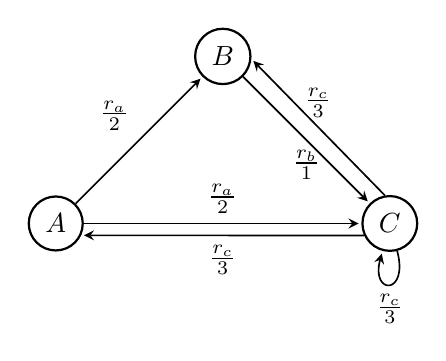
\begin{tikzpicture}[
            > = stealth, % arrow head style
            shorten > = 1pt, % don't touch arrow head to node
            auto,
            node distance = 3cm, % distance between nodes
            semithick % line style
        ]

        \tikzstyle{every state}=[
            draw = black,
            thick,
            fill = white,
            minimum size = 4mm
        ]

        \node[state] (A) {$A$};
        \node[state] (B) [above right of=A] {$B$};
        \node[state] (C) [below right of=B] {$C$};

        \path[->] (A) edge node {$\frac{r_a}{2}$} (B);
        \path[->] (A) edge node {$\frac{r_a}{2}$} (C);
        \path[->] (B) edge [align=center,below] node {$\frac{r_b}{1}$} (C);
        
        % added
        \path[->] (C) edge [loop below] node {$\frac{r_c}{3}$} (C);
        \path[->] (C.100) edge [align=center,above] node {$\frac{r_c}{3}$} (B.-5);
        \path[->] (C.205) edge node {$\frac{r_c}{3}$} (A.-25);

    \end{tikzpicture}
\end{center}

The "Transition Matrix", $T_0$, or weighted matrix is like the link matrix except takes into account the outlinks, $o_i$, for a given edge. $o_i$ is the number of non zero entries in a row, $i$, of the link matrix. And the non zero values of the link matrix are replaced by $\frac{1}{o_i}$ for every element in $T_0$.

\[
T_0 = 
\begin{blockarray}{cccc}
a & b & c \\
\begin{block}{(ccc)c}
  0 & \frac{1}{2} & \frac{1}{2} & a \\
  0 & 0 & 1 & b \\
  \frac{1}{3} & \frac{1}{3} & \frac{1}{3} & c \\
\end{block}
\end{blockarray}
\]


Every row of the "Transition Matrix" sums to $1$, making it a "Right Stochastic Matrix". This matrix can be used to model the surfers movement. Given a starting probability vector \footnote{$\vec{v_a}$ is a row vector because the transition matrix is right stochastic.}, $\vec{v_a}$, with the surfer starting on webpage $a$, you can find the probability that the surfer will be on webpage $a$ on his first visit (which should be $1$),

\iffalse

\[
\vec{v_a} T_0^1 =
\begin{pmatrix}
  1 & 0 & 0 \\
\end{pmatrix}
%
\begin{pmatrix}
  0 & \frac{1}{2} & \frac{1}{2} \\
  0 & 0 & 1  \\
  \frac{1}{3} & \frac{1}{3} & \frac{1}{3} \\
\end{pmatrix}
%
=
%
\begin{pmatrix}
  1 & 0 & 0 \\
\end{pmatrix}
\]

\fi

%
% Example usage, 1 click
%
\[
%
\vec{v_a} T_0^1 =
%
\begin{blockarray}{ccc}
a & b & c \\
\begin{block}{(ccc)}
  1 & 0 & 0 \\
\end{block}
\end{blockarray}
%
\begin{blockarray}{cccc}
a & b & c \\
\begin{block}{(ccc)c}
  0 & \frac{1}{2} & \frac{1}{2} & a \\
  0 & 0 & 1 & b \\
  \frac{1}{3} & \frac{1}{3} & \frac{1}{3} & c \\
\end{block}
\end{blockarray}
%
=
%
\begin{blockarray}{ccc}
a & b & c \\
\begin{block}{(ccc)}
  1 & 0 & 0 \\
\end{block}
\end{blockarray}
\]



Or the different probabilities after $2$ clicks,

\[
\vec{v_a} T_0^2 =
\begin{pmatrix}
  1 & 0 & 0 \\
\end{pmatrix}
%
\begin{pmatrix}
  \frac{1}{6} & \frac{1}{6} & \frac{2}{3} \\
  \frac{1}{3} & \frac{1}{3} & \frac{1}{3}  \\
  \frac{1}{9} & \frac{5}{18} & \frac{11}{18} \\
\end{pmatrix}
%
=
%
\begin{pmatrix}
  \frac{1}{6} & \frac{1}{6} & \frac{2}{3} \\
\end{pmatrix}
\]


Or finally the website ranks, or,

\[
\lim_{k \to\infty} \vec{v_a} T_0^k =
%
\begin{pmatrix}
   \frac{2}{11} & \frac{3}{11} & \frac{6}{11} \\
\end{pmatrix}
\]

Notice the answer comes out to the same one obtained from the system of equations above,

\begin{equation}
	\nonumber r_a = \frac{2}{11}, \, r_b = \frac{3}{11}, \, r_c = \frac{6}{11}
\end{equation}

\[
\vec{r} =
%
\begin{pmatrix}
   \frac{2}{11} & \frac{3}{11} & \frac{6}{11} \\
\end{pmatrix}
\]

$\vec{r}$ will be the same for any starting vector (in this case $\vec{v_a}$). $\vec{r}$ is also the left eigenvector for the eigenvalue, $\lambda = 1$, for the Transition Matrix, $T_0$, created from the "Strongly Connected Webgraph". It is the left eigenvector because the Transition Matrix is right stochastic. If the matrix were left stochastic then $\vec{r}$ would be the right eigenvector for $\lambda = 1$.


%
%	Link Matrix, Probability Matrix, Eigenvector
%


\[
L =
\begin{blockarray}{cccc}
a & b & c \\
\begin{block}{(ccc)c}
  0 & 1 & 1 & a \\
  0 & 0 & 1 & b \\
  1 & 1 & 1 & c \\
\end{block}
\end{blockarray}
%
,
%
T_0 = 
\begin{blockarray}{cccc}
a & b & c \\
\begin{block}{(ccc)c}
  0 & \frac{1}{2} & \frac{1}{2} & a \\
  0 & 0 & 1 & b \\
  \frac{1}{3} & \frac{1}{3} & \frac{1}{3} & c \\
\end{block}
\end{blockarray}
%
,
%
\vec{r} =
%
\begin{pmatrix}
   \frac{2}{11} & \frac{3}{11} & \frac{6}{11} \\
\end{pmatrix}
\]


%
% alpha included
%

\section{Damping Factor}

However if a damping factor is added, $\alpha = 0.15$, is included then the flow equations and graph are changed and the the Transition Matrix, $T_{0.15}$, becomes,

$$
T_{0.15} = 
\left( 0.85 \right)
\begin{pmatrix} 
  0 	& \frac{1}{2} 	& \frac{1}{2}  \\
  0 	& 0 			& 1 		 \\
  \frac{1}{3} 	& \frac{1}{3} 	& \frac{1}{3}
\end{pmatrix}
 + 
\left( 0.15 \right)
\begin{pmatrix} 
  \frac{1}{3} 	& \frac{1}{3} 	& \frac{1}{3} \\
  \frac{1}{3} 	& \frac{1}{3} 	& \frac{1}{3} \\
  \frac{1}{3} 	& \frac{1}{3} 	& \frac{1}{3}
\end{pmatrix}
=
\begin{pmatrix} 
  0.05 	& 0.475 	& 0.475 \\
  0.05 	& 0.05 	& 0.09 \\
  0.33 \dots 	&  0.33 \dots 	&  0.33 \dots
\end{pmatrix}
$$

Or for different values of $\alpha$,

$$
T_{\alpha} = 
\left( 1 - \alpha \right)
\begin{pmatrix} 
  0 	& \frac{1}{2} 	& \frac{1}{2}  \\
  0 	& 0 			& 1 		 \\
  \frac{1}{3} 	& \frac{1}{3} 	& \frac{1}{3}
\end{pmatrix}
 + 
\left( \alpha \right)
\begin{pmatrix} 
  \frac{1}{3} 	& \frac{1}{3} 	& \frac{1}{3} \\
  \frac{1}{3} 	& \frac{1}{3} 	& \frac{1}{3} \\
  \frac{1}{3} 	& \frac{1}{3} 	& \frac{1}{3}
\end{pmatrix}
$$

Adding $\alpha$ makes it possible for the surfer to jump to a random website in the graph.

%
%	Question 1 Answer
%

\section{Question 1 Answer}
1.	(25/25 points) Consider the following web pages and the set of web pages that they link to:
Page A points to pages B and C.
Page B points to page C.
All other pages have no outgoing links.
Apply the PageRank algorithm to this subgraph of pages. Assume $\alpha$ = 0.15. Simulate the algorithm for three iterations. 

If you choose the starting vector, $\vec{v}$, to be the left eigenvector of $T_{0.15}$ corresponding to the eigenvalue $\lambda = 1$, then the probabilities will not change for each iteration.

% Web Graph
\begin{center}
	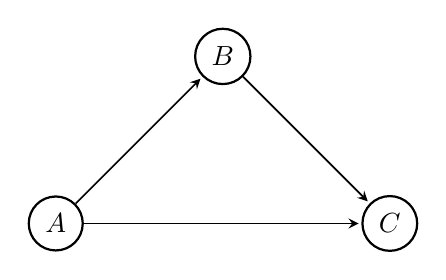
\begin{tikzpicture}[
            > = stealth, % arrow head style
            shorten > = 1pt, % don't touch arrow head to node
            auto,
            node distance = 3cm, % distance between nodes
            semithick % line style
        ]

        \tikzstyle{every state}=[
            draw = black,
            thick,
            fill = white,
            minimum size = 4mm
        ]

        \node[state] (A) {$A$};
        \node[state] (B) [above right of=A] {$B$};
        \node[state] (C) [below right of=B] {$C$};

        \path[->] (A) edge node {} (B);
        \path[->] (A) edge node {} (C);
        \path[->] (B) edge node {} (C);


        %\draw[red, dashed] (1, 2) -- (1, -2);
    \end{tikzpicture}
\end{center}


$$
T_{0.15}
=
\begin{pmatrix} 
  0.05 	& 0.475 	& 0.475 \\
  0.05 	& 0.05 	& 0.09 \\
  0.33 \dots 	&  0.33 \dots 	&  0.33 \dots
\end{pmatrix}
$$


\begin{equation}
\nonumber \vec{v} \approx
\begin{pmatrix}
   0.19757929 &  0.28155074 & 0.52086996 \\
\end{pmatrix}
\end{equation}

Then for $k=3$,

$$
\vec{r} = \vec{v} T_{0.15}^3 = \vec{v} \approx 
%
\begin{blockarray}{ccc}
a & b & c \\
\begin{block}{(ccc)}
  0.19757929 &  0.28155074 & 0.52086996\\
\end{block}
\end{blockarray}
$$

\iffalse

Which would correspond to the maximum right eigenvector of the matrix P below. However if the damping factor, $alpha$, is included then the equations and graph are changed.

% Damping Web Graph
\begin{center} Damped Web Graph \end{center}

\begin{center}
	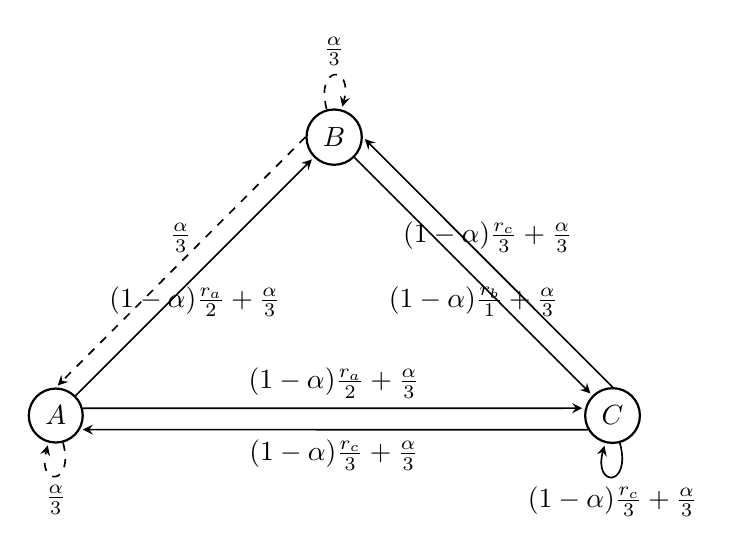
\begin{tikzpicture}[
            > = stealth, % arrow head style
            shorten > = 1pt, % don't touch arrow head to node
            auto,
            node distance = 5cm, % distance between nodes
            semithick % line style
        ]

        \tikzstyle{every state}=[
            draw = black,
            thick,
            fill = white,
            minimum size = 4mm
        ]

        \node[state] (A) {$A$};
        \node[state] (B) [above right of=A] {$B$};
        \node[state] (C) [below right of=B] {$C$};

		% A paths
        \path[->] (A) edge [align=center,below] node {$(1-\alpha)\frac{r_a}{2} + \frac{\alpha}{3}$} (B);
        \path[->] (A.15) edge node {$(1-\alpha)\frac{r_a}{2} + \frac{\alpha}{3}$} (C.165);
        
        \path[->, dashed] (A) edge [loop below] node {$\frac{\alpha}{3}$} (A);
        
        % B paths
        \path[->] (B) edge [align=center,below] node {$(1-\alpha)\frac{r_b}{1} + \frac{\alpha}{3}$} (C);
        
        \path[->, dashed] (B.180) edge [align=center,above] node {$\frac{\alpha}{3}$} (A.90);
        \path[->, dashed] (B) edge [loop above] node {$\frac{\alpha}{3}$} (B);
        
        % C paths
        \path[->] (C) edge [loop below] node {$(1-\alpha)\frac{r_c}{3} + \frac{\alpha}{3}$} (C);
        \path[->] (C.90) edge [align=center,above] node {$(1-\alpha)\frac{r_c}{3} + \frac{\alpha}{3}$} (B.0);
        \path[->] (C.210) edge node {$(1-\alpha)\frac{r_c}{3} + \frac{\alpha}{3}$} (A.-30);

    \end{tikzpicture}
\end{center}

%
% The new flow equations of the damped graph
%
The new flow equations of the damped graph,

% flow equations
Flow Equations
\begin{equation}
	r_a =  (1-\alpha)\frac{r_c}{3} + \alpha
\end{equation}

\begin{equation}
	r_b = (1-\alpha)\frac{r_a}{2} + (1-\alpha)\frac{r_c}{3} + \alpha
\end{equation}

\begin{equation}
	r_c = (1-\alpha)\frac{r_a}{2} + (1-\alpha)\frac{r_b}{1} + (1-\alpha)\frac{r_c}{3} + \alpha
\end{equation}

\begin{equation}
	r_a + r_b + r_c = 1
\end{equation}


%
%	Link Matrix
%

Link Matrix,
\[
\begin{blockarray}{cccc}
a & b & c \\
\begin{block}{(ccc)c}
  0 & 1 & 1 & a \\
  0 & 0 & 1 & b \\
  0 & 0 & 0 & c \\
\end{block}
\end{blockarray}
\]

Row/Right Stochastic Transition Probability Matrix, $P$, 

$$
P = 
\left( 0.85 \right)
\begin{pmatrix} 
  0 	& \frac{1}{2} 	& \frac{1}{2}  \\
  0 	& 0 			& 1 		 \\
  \frac{1}{3} 	& \frac{1}{3} 	& \frac{1}{3}
\end{pmatrix}
 + 
\left( 0.15 \right)
\begin{pmatrix} 
  \frac{1}{3} 	& \frac{1}{3} 	& \frac{1}{3} \\
  \frac{1}{3} 	& \frac{1}{3} 	& \frac{1}{3} \\
  \frac{1}{3} 	& \frac{1}{3} 	& \frac{1}{3}
\end{pmatrix}
=
\begin{pmatrix} 
  0.05 	& 0.475 	& 0.475 \\
  0.05 	& 0.05 	& 0.09 \\
  0.33 \dots 	&  0.33 \dots 	&  0.33 \dots
\end{pmatrix}
$$


\fi

\end{document}